\documentclass[a4paper,11pt]{article}
\usepackage{array}
\usepackage{tabularx}
\usepackage{booktabs}
\usepackage{graphicx}
\usepackage{framed}
\newcommand{\ra}[1]{\renewcommand{\arraystretch}{#1}}
\newcommand{\specialcell}[1]{\begin{tabular}{@{}c@{}#1\end{tabular}}}
\newcommand{\CS}{C\nolinebreak\hspace{-.05em}\raisebox{.6ex}{\tiny\bf \#}}
% define the title
\author{ButterFree}
\title{Calendar System}
\begin{document}
% generates the title
\maketitle
% insert the table of contents
\tableofcontents
\newpage
\section{Revision Table}
\begin{table*}[ht]\centering
  \ra{1.3}
  \begin{tabularx}{\textwidth}{@{}rX@{}}
    \toprule
    \textbf{Week} & \textbf{Changes} \\\hline
    Week 39 & Revision table added\newline  
    		UML Package Diagram added\newline
    		Design Decisions added\newline
    		!!--- Use case reviewed ---!!\\\hline
    Week 40 & Nothing yet\\
    \bottomrule
  \end{tabularx}
  \caption{Revision table shows what has been changed or added and at what time.}
  \label{glossary}\centering
\end{table*}
\newpage
\section{Vision}
Our vision for the Calendar System is to create an easy to use multiuser
schedule for organizing meetings. We realise that multiple similar services
already exist. What we want to do, is create a bridge between calendar systems. We want people, who use different calendar applications, to plan together.
\newpage

\section{Use cases}
\begin{table*}[ht]\centering
  \ra{1.3}
  \begin{tabularx}{\textwidth}{@{}rXXl@{}}\toprule
    \textbf{ID} & \textbf{Description} & \textbf{Notes} & \textbf{Priority} \\\hline
    1 & The user creates an appointment with another user.             & The
    target can either be in our calendar system or in another iCal compatible
    system. & High \\\hline
    2 & The user accepts an invite to an appointment with another user & Same
    as above
    & High \\
    \bottomrule
  \end{tabularx}
  \caption{Our use cases}
  \label{usecases}\centering% 
\end{table*}
\subsection{Use case 1}
The user wish to create an appointment with another user. The user must first create the appointment in his own calendar system. He then selects the event on our website, and chooses "Invite Attendee". A list of contacts are shown, and the user can select on ore more contacts he wants to invite. The user can add a text to the invitation. The people invited will be notified. The user will receive notification when each invited attendee accepts or declines.
\subsection{Use case 2}
The user has gotten an invitation to an appointment with another user, and he wants to reply.
The user logs on to our website, and finds the invitation in his notifications. The user can press either 'Accept' or 'Decline'. The user can add a text to his reply.
\newpage

\section{Use Cases UML Diagram}
\begin{figure}[h!]
  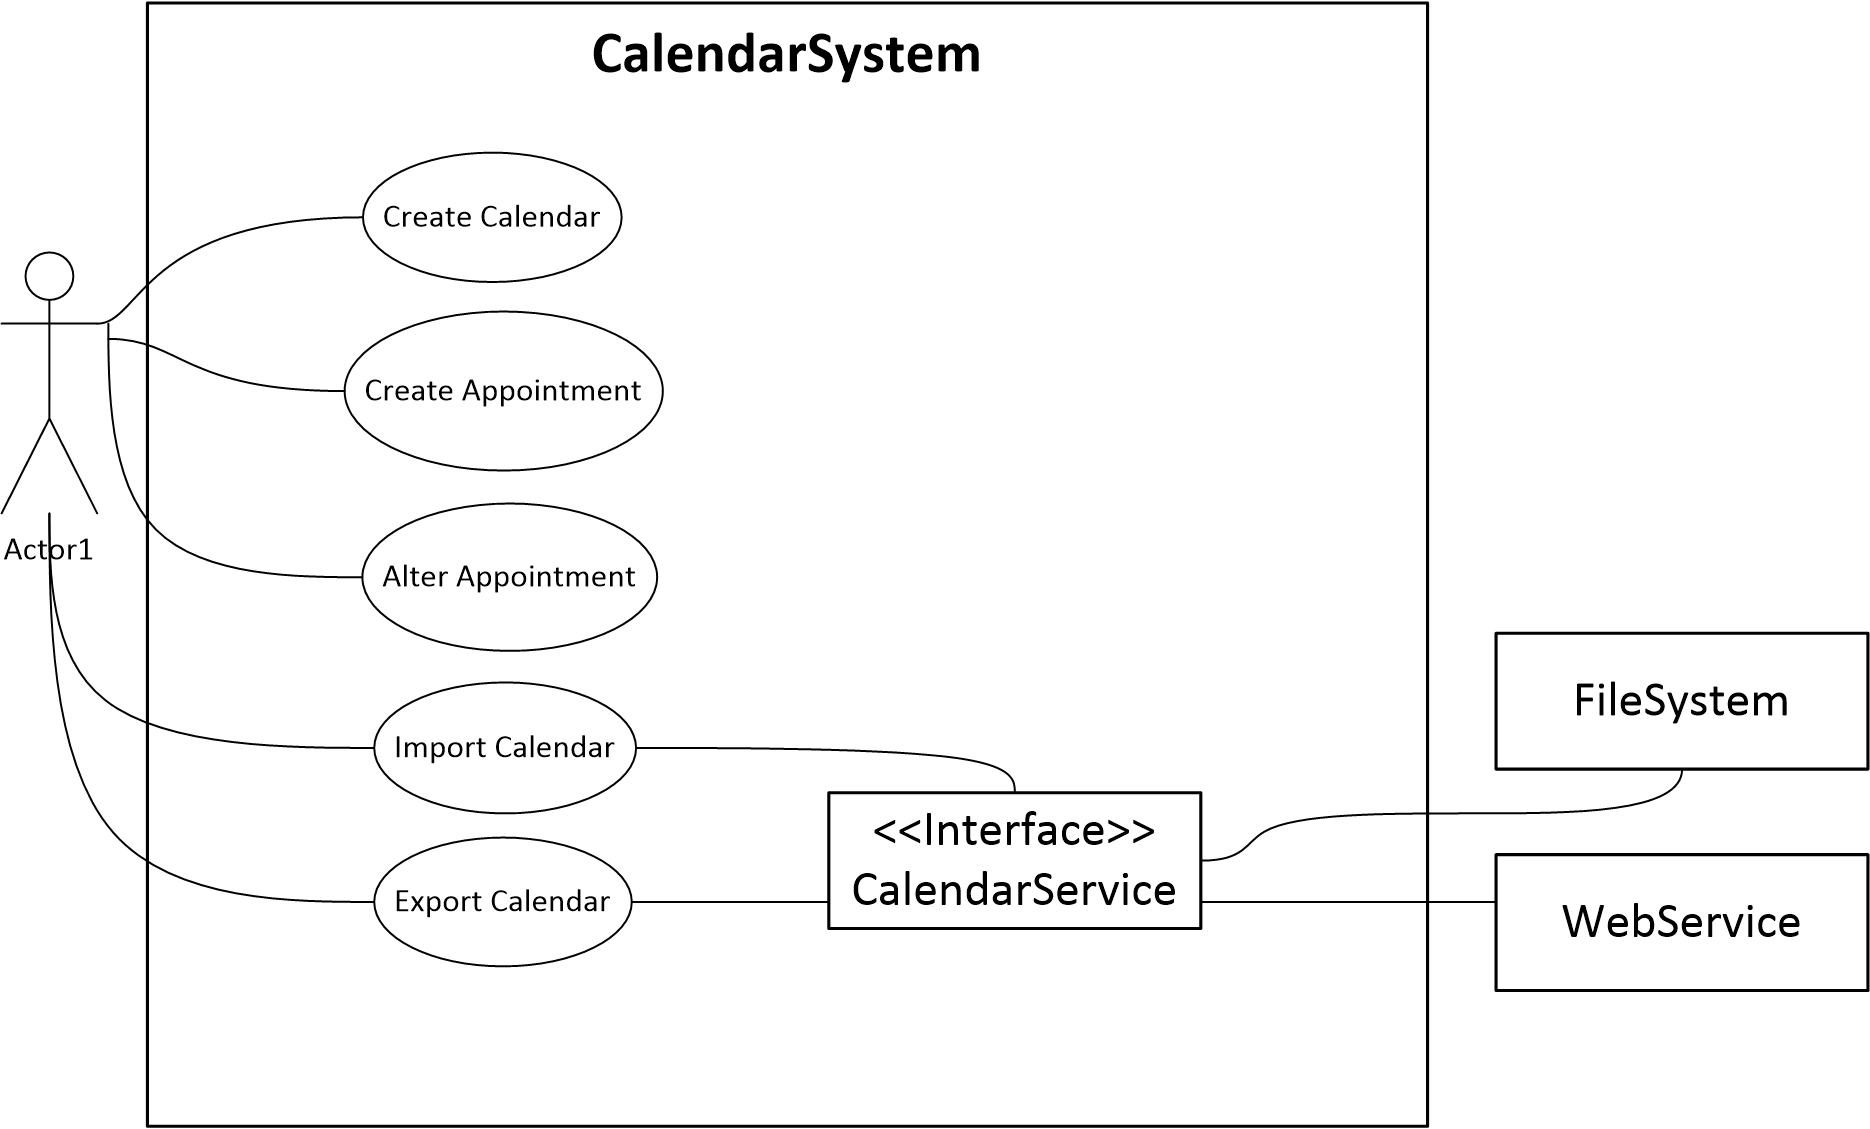
\includegraphics[width=\textwidth,natwidth=839,natheight=508]{illustrations/UseCaseUML.png}
  \caption{The UML diagram for our use cases}
\end{figure}
\newpage

\section{Glossary}
\begin{table*}[ht]\centering
  \ra{1.3}
  \begin{tabularx}{\textwidth}{@{}rX@{}}
    \toprule
    \textbf{Word} & \textbf{Description} \\\hline
    Appointment & An appointment with the data that can be stored in the iCal format \\\hline
    iCal 		& See iCalendar \\\hline
    iCalendar	& iCalendar is a computer file format which allows Internet users to send meeting requests and tasks to other Internet users \\\hline
    Share       & Send an appointment to another user via the iCal format \\\hline
    User        & A user of an iCal compatible system. When several users are mentioned the first one is the user of our system\\
    \bottomrule
  \end{tabularx}
  \caption{Our glossary explaining the terms we use}
%  \label{glossary}\centering
\end{table*}
\newpage

\section{Supplementary Requirements}
In this section we will cover any supplementary requirements.
\subsection{Functionality}
\textit{No additional requirements.}
\subsection{Usability}
\textit{No additional requirements.}
\subsection{Reliability}
\begin{itemize}
  \item Our system must be available to our users at least 90\% of the time
\end{itemize}
\subsection{Performance}
\begin{itemize}
  \item Our system must respond in less than 1 sec in 90\% of the cases.
    (External system are out of our control, and this time is therefore
    subtracted)
\end{itemize}
\subsection{Supportability}
\begin{itemize}
  \item Compatible with all iCal-systems.
\end{itemize}
\newpage

\section{Domain Model}
\begin{figure}[h!]
  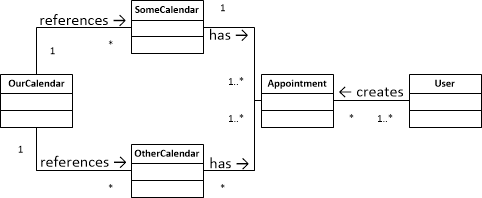
\includegraphics[width=\textwidth,natwidth=682,natheight=757]{illustrations/DomainModel.png}
  \caption{Model illustrating our domain and its relations}
\end{figure}
\newpage

\section{System Sequence Diagram}
\begin{figure}[h!]
  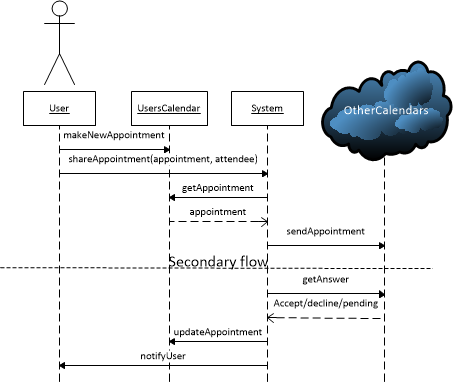
\includegraphics[width=\textwidth,natwidth=266,natheight=228]{illustrations/SSD.png}
  \caption{The sequence diagram for our system}
\end{figure}
\newpage

\section{Operation Contract Template}
  \subsection{OCT 1}
    \begin{table*}[ht]\centering
      \ra{1.3}
      \begin{tabularx}{\textwidth}{@{}|rX|@{}}\hline
        \textbf{Operation:}        & AddCalendar(Calendar) \\
        \textbf{Cross references:} & SSD diagram\\
        \textbf{Preconditions:}    & Program is running. No existing calendars are required. \\
        \textbf{Postconditions:}   & A calendar now exists in the system. \\\hline
      \end{tabularx}
    \end{table*}
  \subsection{OCT 2}
    \begin{table*}[ht]\centering
      \ra{1.3}
      \begin{tabularx}{\textwidth}{@{}|rX|@{}}\hline
        \textbf{Operation:}        & GetEvents(Calendar, TimePeriod)()\\
        \textbf{Cross references:} & SSD diagram \\
        \textbf{Preconditions:}    & Program holds the calendar the user wish to view. \\
        \textbf{Postconditions:}   & The program shows events from the selected calendar within the given time period. \\\hline
      \end{tabularx}
    \end{table*}
  \subsection{OCT 3}
    \begin{table*}[ht]\centering
      \ra{1.3}
      \begin{tabularx}{\textwidth}{@{}|rX|@{}}\hline
        \textbf{Operation:}        & AddEvent(Calendar, Event)()\\
        \textbf{Cross references:} & SSD diagram \\
        \textbf{Preconditions:}    & Program holds the calendar the user wish to add an event to. \\
        \textbf{Postconditions:}   & Event is saved to the calendar. The program shows events from the selected calendar within the given time period. \\\hline
      \end{tabularx}
    \end{table*}
\newpage

\section{Design Class Diagram}
\begin{figure}[h!]
  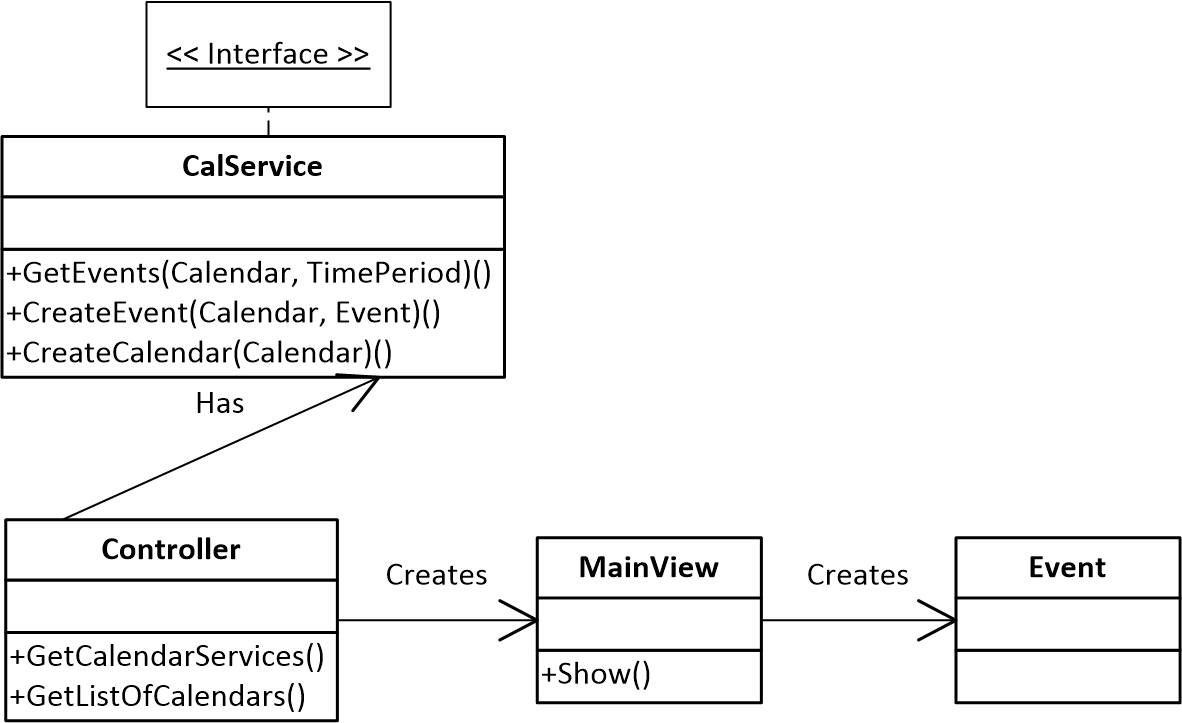
\includegraphics[width=\textwidth,natwidth=1073,natheight=976]{illustrations/DesignClassDiagram.png}
  \caption{The Design Class Diagram for our system}
\end{figure}
\newpage
\section{UML Package Diagram}
\begin{figure}[h!]
  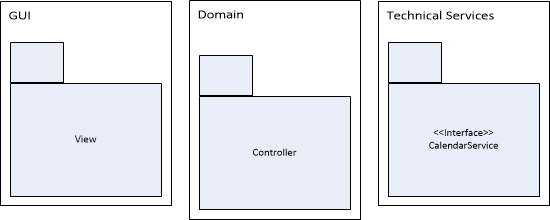
\includegraphics[width=\textwidth,natwidth=1717,natheight=685]{illustrations/UMLPackageDiagram.png}
  \caption{UML Package Diagram}
\end{figure}
\newpage
\section{Class Diagram}
\begin{figure}[h!]
  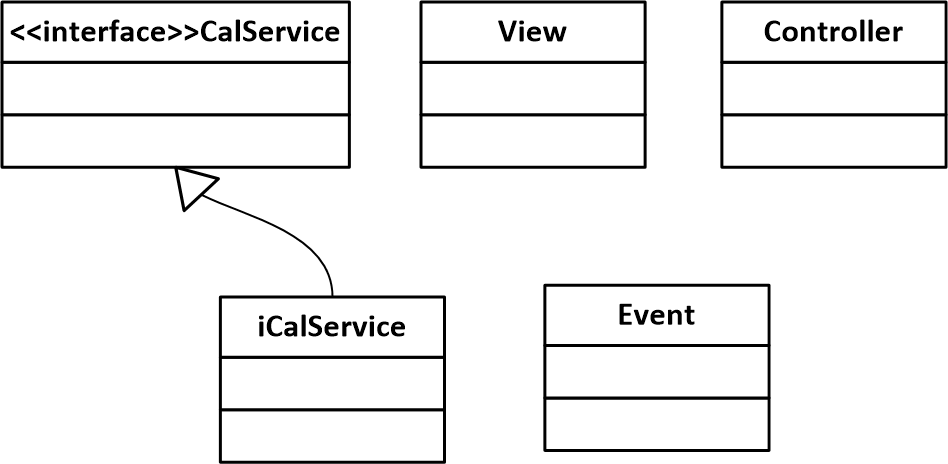
\includegraphics[width=\textwidth,natwidth=948,natheight=464]{illustrations/classdiagram.png}
  \caption{The class diagram for our system}
\end{figure}
\newpage

\section{Design Decisions}
We have chosen to use the MVC design pattern for our \CS application. For the overall build we will be using the client-server pattern.

The client-server pattern is the obvious choice since we are building a client which will be communicating with one or more servers.

MVC separates the three parts of our client, and makes it easy to switch one part. This also makes it easy for us to wait with the visual part and focus on the backbone of our system.

\begin{figure}[h!]
  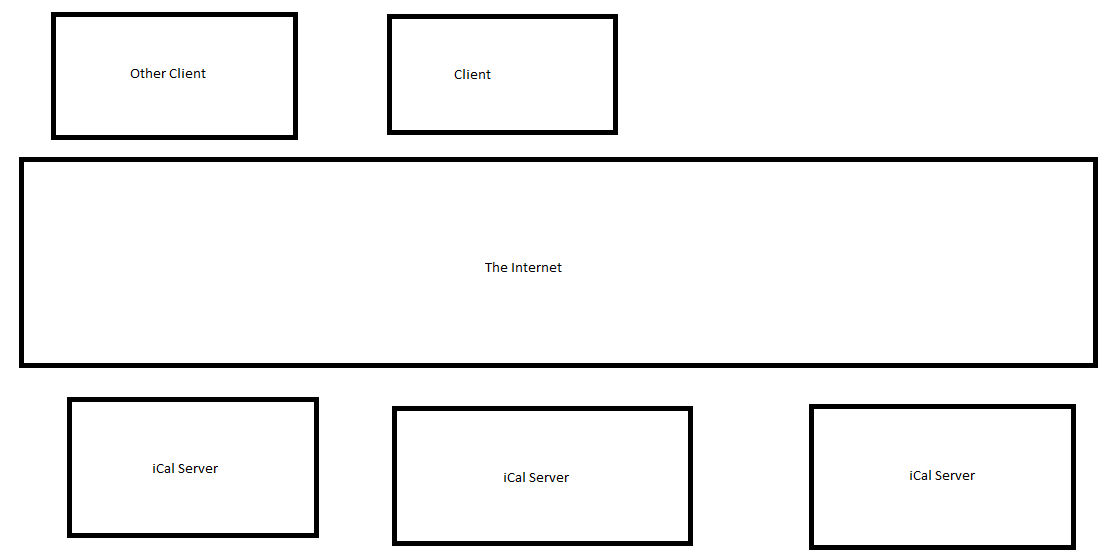
\includegraphics[width=\textwidth,natwidth=1109,natheight=559]{illustrations/PhysicalModel.png}
  \caption{Physical model of our build.}
\end{figure}

\newpage
\section{GRASP}
\subsection{Creator}
Our Main View (GUI class) will create sub views as the user explore our program. These will be held by the Main View.

\subsection{Expert}
Our Controller package contains an object which is responsible for calendars. It holds a list of CalendarServices and a list of Calendars.

\subsection{Low Coupling}
We keep our coupling low by using an interface we call CalenderService. If you write a class, which implements our interface, it can be used as a calendar handler. This might be iCal or simply a calender written to the file system. 
We also use the MVC pattern which assigns clear responsibilities and makes it easy to switch one class with a different version.

\subsection{Controller}
We have a Controller package containing a Controller class. This class has the main responsibilities, error handling and it is used to couple the Model and View.

\subsection{High Cohesion}
Good examples of high cohesion are our Event class and CalenderService interface. They both have very specific and simple tasks to fulfill. 

\newpage
\section{SCRUM}
We used Pivotal Tracker as a tool for SCRUM.\\
https://www.pivotaltracker.com/projects/678161\\

\subsection{Definition of Done}
We need to define when a story is done. We have chosen that a story can not be
marked as done before it fulfilled the following: \\
- Proper documentation has been written
- Tests have been written and they they must not fail
- New code must not break previously written tests

\newpage

\section{Collaboration Diagram}
A Sequence diagram shows interaction in the correct sequence whereas Collaboration digram does not.
Collaboration diagrams are easier to sketch on a whiteboard, where Sequence diagrams requires a lot of space.
A Sequence diagram has a much more simple and easy to remember notation.

\begin{figure}[h!]
  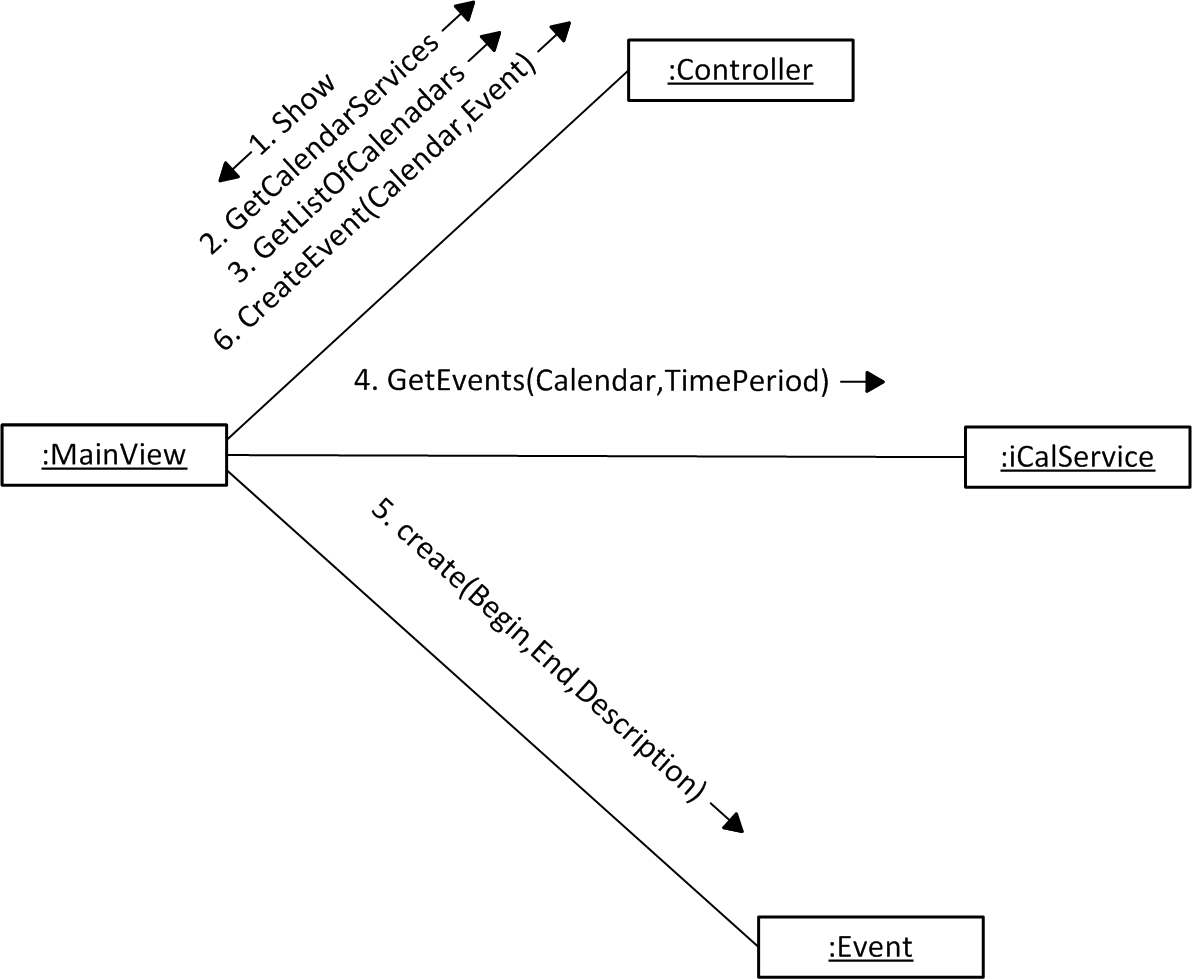
\includegraphics[width=\textwidth,natwidth=1192,natheight=979]{illustrations/CollaborationDiagram.png}
  \caption{Collaboration diagram}
\end{figure}
\newpage
\end{document}